%%%%%%%%%%%%%%%%%%%%%%%%%%%%%%%%%%%%%%%%%%%%%%%%%%%%%%%%%%%%%%%%%%
%%%%%%%% ICML 2013 EXAMPLE LATEX SUBMISSION FILE %%%%%%%%%%%%%%%%%
%%%%%%%%%%%%%%%%%%%%%%%%%%%%%%%%%%%%%%%%%%%%%%%%%%%%%%%%%%%%%%%%%%

% Use the following line _only_ if you're still using LaTeX 2.09.
%\documentstyle[icml2013,epsf,natbib]{article}
% If you rely on Latex2e packages, like most moden people use this:
\documentclass[11pt]{article}

% For figures
\usepackage{graphicx} % more modern
%\usepackage{epsfig} % less modern
\usepackage{subfigure}


% For math symbol
\usepackage{amsmath,amsfonts,amssymb}

% For theorem
\usepackage{amsthm}

% For citations
\usepackage{natbib}

% For algorithms
\usepackage{algorithm}
\usepackage{algorithmic}

% For appendix
% \usepackage[title,titletoc,toc]{appendix}

% For graphical model
% \usepackage{tikz}
% \usetikzlibrary{fit,positioning}
% \usetikzlibrary{arrows,shapes}
% As of 2011, we use the hyperref package to produce hyperlinks in the
% resulting PDF.  If this breaks your system, please commend out the
% following usepackage line and replace \usepackage{icml2013} with
% \usepackage[nohyperref]{icml2013} above.
\usepackage{hyperref}

% Packages hyperref and algorithmic misbehave sometimes.  We can fix
% this with the following command.
\newcommand{\theHalgorithm}{\arabic{algorithm}}
\newcommand{\trans}{\top}
\newcommand{\bm}{\mathbf}

\newcommand{\comment}[1]{}

% theorem macro
\newtheorem{thm}{Theorem}
\newtheorem{lem}[thm]{Lemma}

% Employ the following version of the ``usepackage'' statement for
% submitting the draft version of the paper for review.  This will set
% the note in the first column to ``Under review.  Do not distribute.''
% \usepackage{icml2013}
% \usepackage[accepted]{icml2013}
% Employ this version of the ``usepackage'' statement after the paper has
% been accepted, when creating the final version.  This will set the
% note in the first column to ``Proceedings of the...''
% \usepackage[accepted]{icml2013}

\usepackage{fullpage}
\usepackage{xcolor}
% The \icmltitle you define below is probably too long as a header.
% Therefore, a short form for the running title is supplied here:
% \icmltitlerunning{Submission and Formatting Instructions for ICML 2013}


\title{Experiments}

\begin{document}
\maketitle

%\twocolumn[
%\icmltitle{}

% It is OKAY to include author information, even for blind
% submissions: the style file will automatically remove it for you
% unless you've provided the [accepted] option to the icml2013
% package.

% \icmlauthor{Your Name}{email@yourdomain.edu}
% \icmladdress{Your Fantastic Institute,
%            314159 Pi St., Palo Alto, CA 94306 USA}
%\icmlauthor{Your CoAuthor's Name}{email@coauthordomain.edu}
%\icmladdress{Their Fantastic Institute,
%            27182 Exp St., Toronto, ON M6H 2T1 CANADA}

% You may provide any keywords that you
% find helpful for describing your paper; these are used to populate
% the "keywords" metadata in the PDF but will not be shown in the document

%\icmlkeywords{exponential family harmonium, markov random fields, Deep Boltzmann Machine, Gaussian Integral trick}

%\vskip 0.3in
%]

%\section{Multiview Latent Variable Models}

\section{Synthetic Dataset}

\texttt{More mathematical formula}

To verify the proposed algorithm, we compared with EM for mixture of Gaussians and spectral algorithm for mixture of spherical Gaussians~\citep{Hsu13}. The assumption in~\citep{Hsu13} is very restricted, the means of the each Gaussian component should span a $k$-dimension subpsace, where $k$ is number of components. Meanwhile, each component should be a spherical Gaussian. We also compared with another \emph{nonparametric} spectral algorithms propsed by~\citep{Hiroyuki10} which uses histgram to approximate the conditional distribution. It could be thought as a special case of our method using delta kernel. It is predictable that their performance is not comparable to others because of the inferior histgram comparing to smooth kernel, the error is about $10$ times to EM method. So that, we didn't plot it in the figures.

We generated synthetic data from the mixture models in four different settings, i.e., each view with different/same Gaussian/Gamma and Gaussian conditional distributions.  \textcolor{red}{In the Gamma/Gaussian mixture, we chose parameters to make the Gamma distribution more skew in latter two views while in the first view similar to Gaussian.} \textcolor{blue}{In the Gamma/Gaussian mixture, we chose parameters to make the Gamma distribution more skew}. For all the setting, we set the covariance of Gaussians be diagonal. The parameters for Gaussian and Gamma distributions are predefined to make sure they are not overlapped to much in the sense of the ratio of the distance between the mode of classes to the variance within the classes, i.e., for each pair of clusters, $\frac{(\mu_1 - \mu_2)^2}{\sum_{i = 1}^1\sigma_i^2}$ is big enough where $\mu = \frac{(\alpha-1)}{\beta}$ and $\sigma^2 = \frac{\alpha}{\beta^2}$ in Gamma distribution. We also varied the number of observations $n$, from $50$ to $100, 000$,  and components $k$ in range $[2,3,4,8]$ in experiments to illustrate the convergence property of our algorithm. The mixture proportions are set to be $p_i = \frac{2i}{k(k+1)}, i\in\{1, \ldots, k\}$ which is highly unbalanced. It is worth to remark that when $k$ becomes large but $n$ is small, such setting is extremly difficult since only a little data will be generated from the first several clusters. For each $n,k$ in each setting, we randomly sampled 10 sets of instances from the model for training.

For EM algorithm, since it is not guaranteed to get the global solutions each trial, we repeated it $10$ times with random initialization and added regularization term to make sure the covariance parameters is valid. We selected the best kernel bandwidth for each view by evaluated on separated generated datasets. We measured the performance of algorithms by the $l2$-norm $||\sum_h p(x_i|h)p(h) - \sum_h\hat{p}(x_i|h)\hat{p}(h)||_2$ to the ground-truth marginal distribution of each view. 

The results are plotted below. It is clear that both the nonparametric method and EM converge rapidly with the data increment in all experiments setting. 

In mixture of Gaussian setting, the EM algorithm is best because the setting is fully satisfied to its assumption. While the spectral learning algorithm for sphereical Gaussian didn't perform well since the assumption for the method is too restrict. It is reasonable that our nonparametric is a little bit worse than EM algorithm because of the complexity nonparametric form of probability distribution.

In the mixture of Gaussian/Gamma setting, the EM algorithm is good when data is less. However, our nonparametric spectral algorithm provided the best results when sample size is large enough. This phenomena demonstrated the trade-off between model complexity and sample size. 

\begin{figure}
	\subfigure[View 1]{
		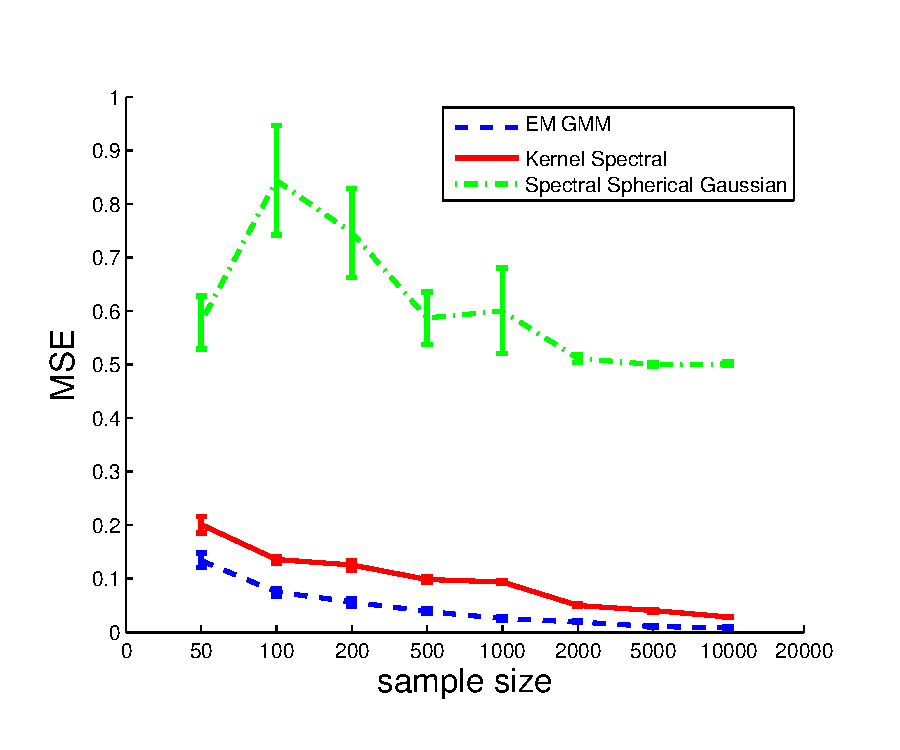
\includegraphics[width=0.32\textwidth]{figure/diff_gauss_k_2_view_3.pdf}
	}
	\subfigure[View 2]{
		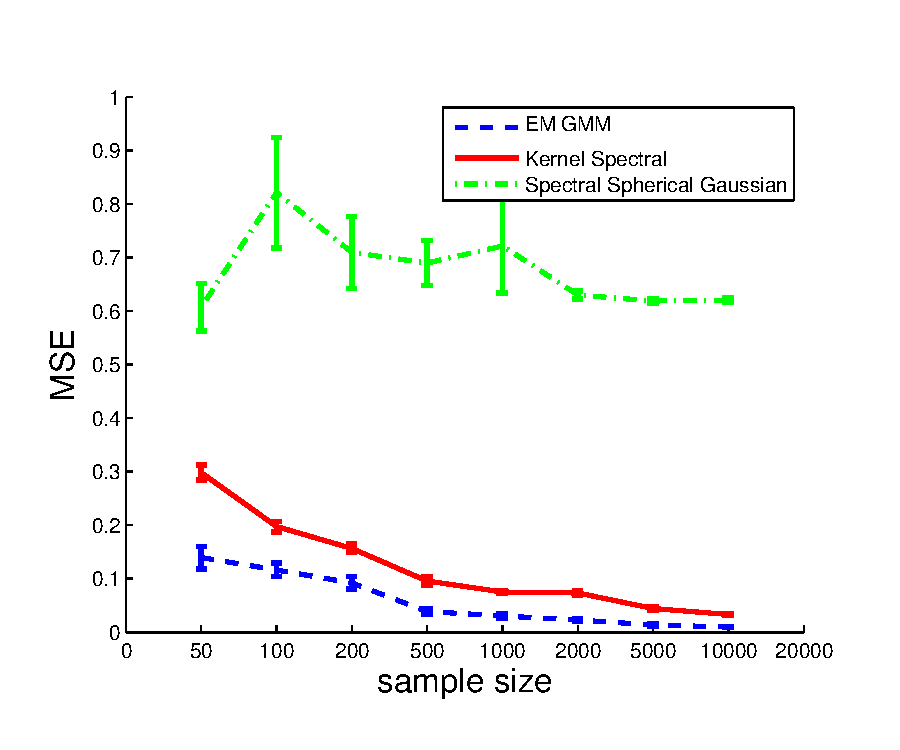
\includegraphics[width=0.32\textwidth]{figure/diff_gauss_k_2_view_2.pdf}
	}
	\subfigure[View 3]{
		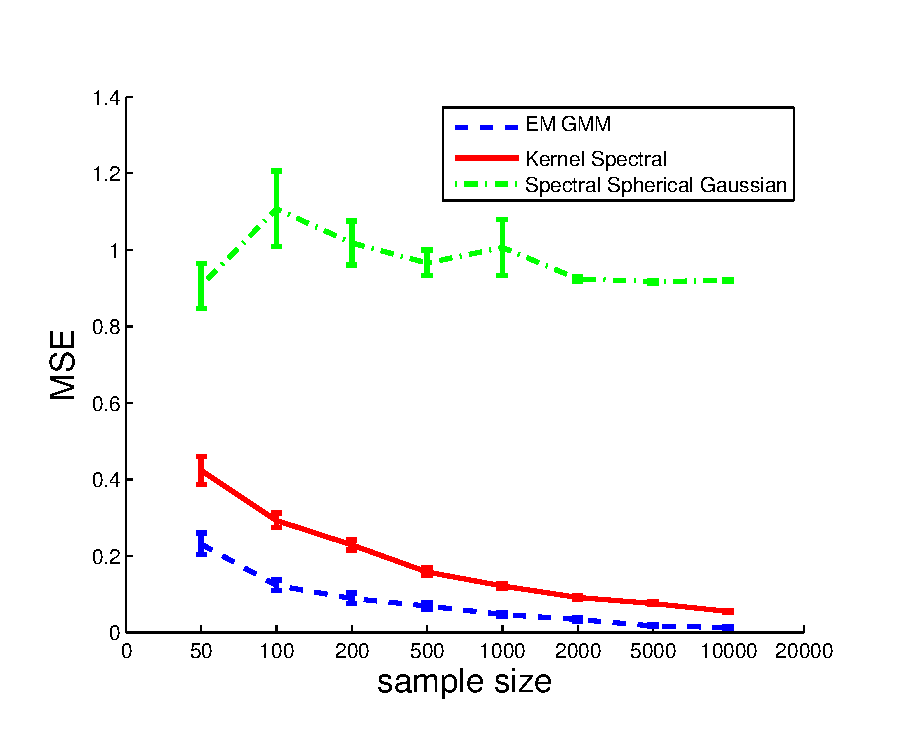
\includegraphics[width=0.32\textwidth]{figure/diff_gauss_k_2_view_1.pdf}
	}
\caption{The empirical results on synthetic dataset with different 2 Gaussian components in each view measured by the $l2$-norm between marginal distribution and ground-truth for each view.}
\end{figure}


\begin{figure}
	\subfigure[View 1]{
		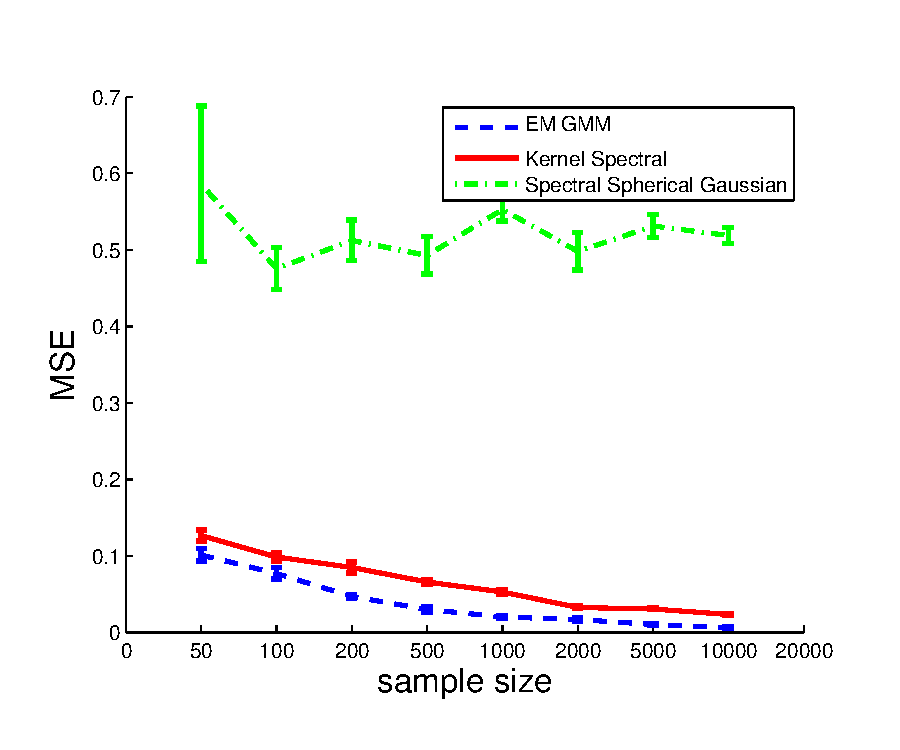
\includegraphics[width=0.32\textwidth]{figure/diff_gauss_k_3_view_3.pdf}
	}
	\subfigure[View 2]{
		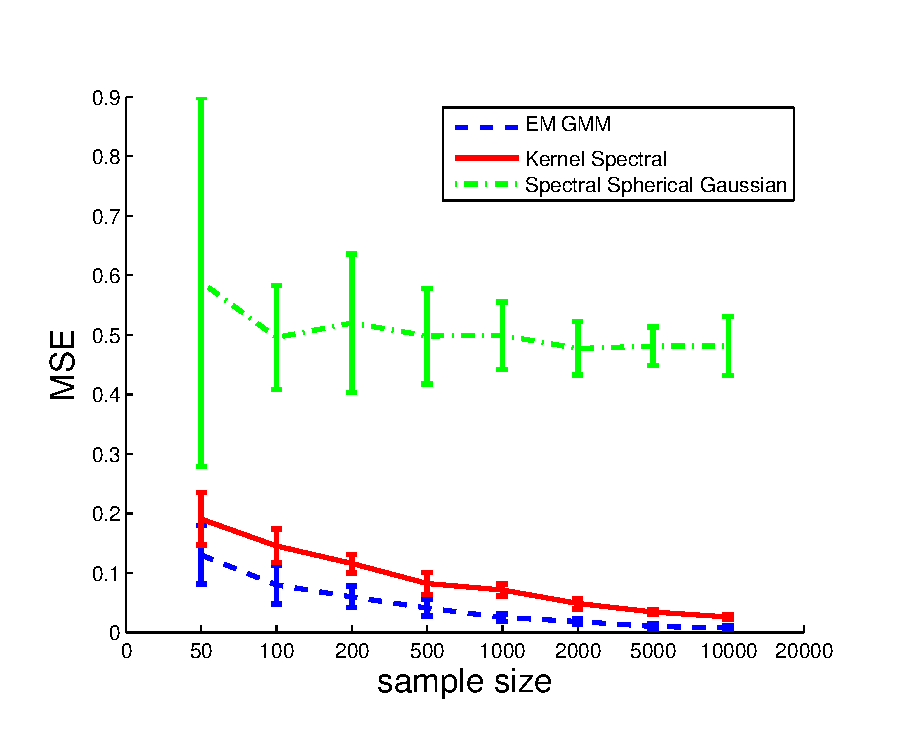
\includegraphics[width=0.32\textwidth]{figure/diff_gauss_k_3_view_2.pdf}
	}
	\subfigure[View 3]{
		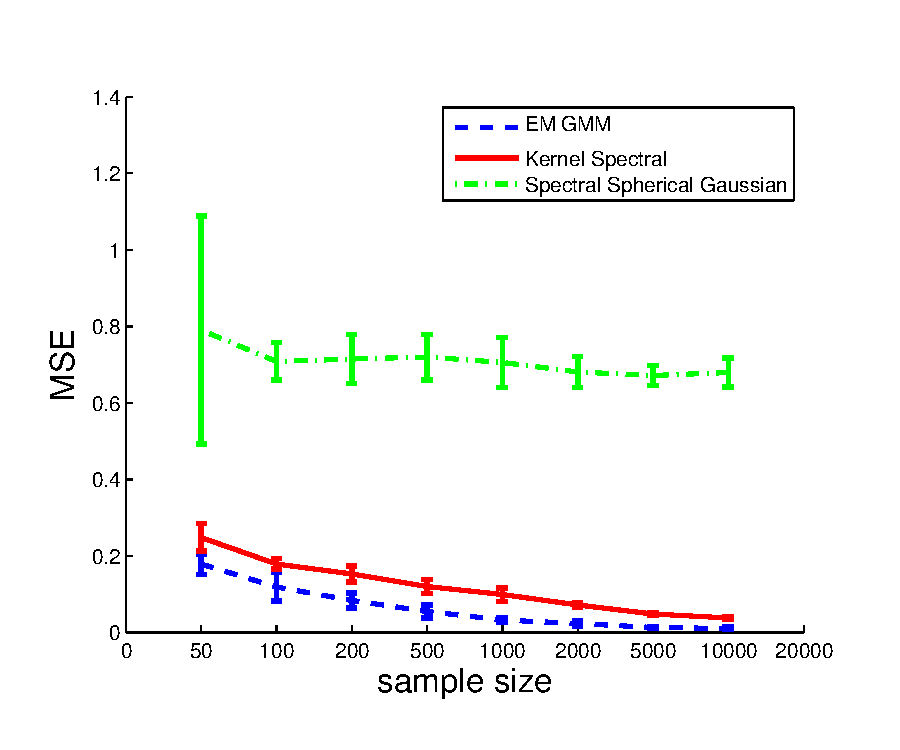
\includegraphics[width=0.32\textwidth]{figure/diff_gauss_k_3_view_1.pdf}
	}
\caption{The empirical results on synthetic dataset with different 3 Gaussian components in each view measured by the $l2$-norm between marginal distribution and ground-truth for each view.}
\end{figure}

\begin{figure}
	\subfigure[View 1]{
		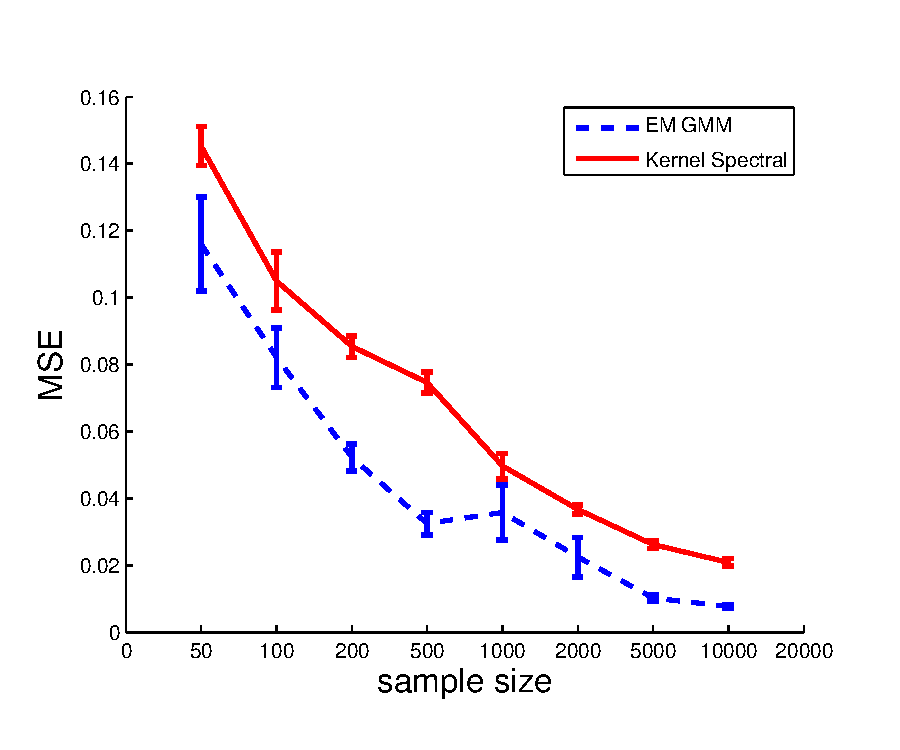
\includegraphics[width=0.32\textwidth]{figure/diff_gauss_k_4_view_3.pdf}
	}
	\subfigure[View 2]{
		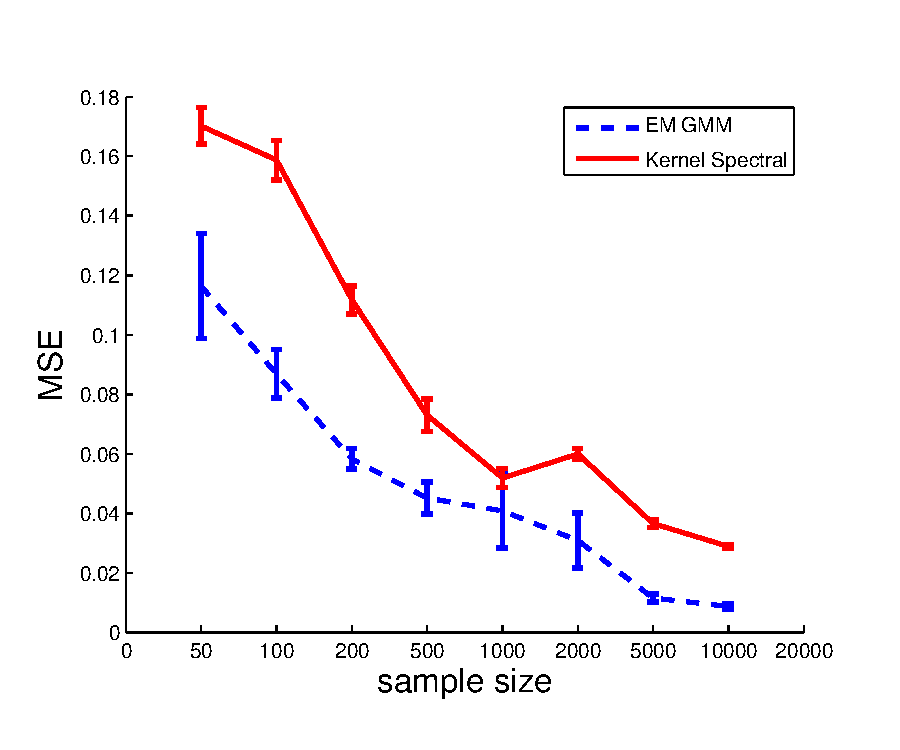
\includegraphics[width=0.32\textwidth]{figure/diff_gauss_k_4_view_2.pdf}
	}
	\subfigure[View 3]{
		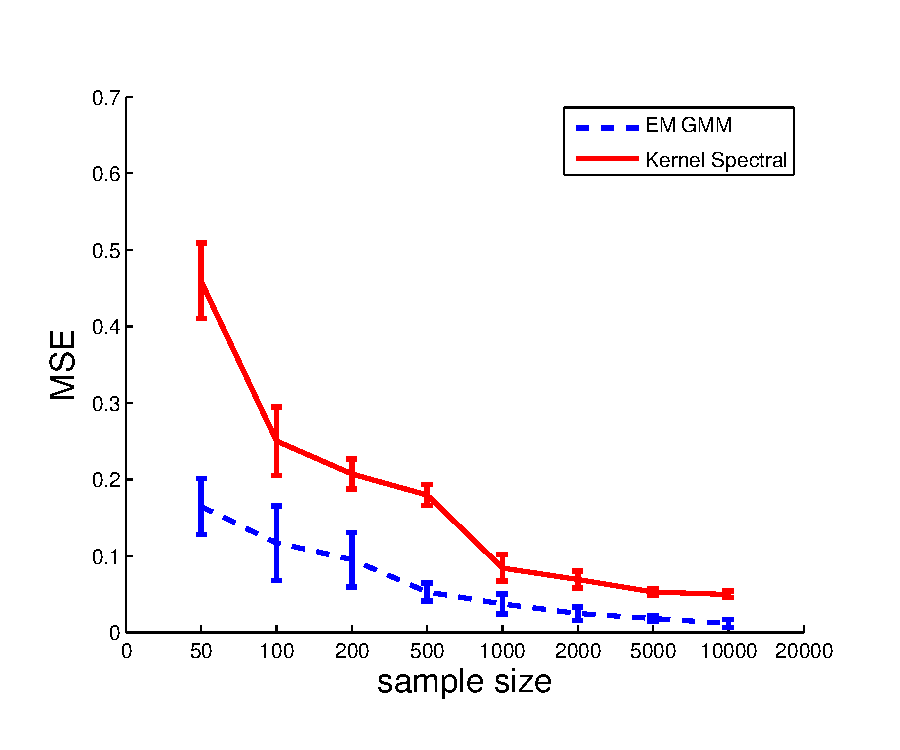
\includegraphics[width=0.32\textwidth]{figure/diff_gauss_k_4_view_1.pdf}
	}
\caption{The empirical results on synthetic dataset with different 4 Gaussian components in each view measured by the $l2$-norm between marginal distribution and ground-truth for each view.}
\end{figure}

\begin{figure}
	\subfigure[View 1]{
		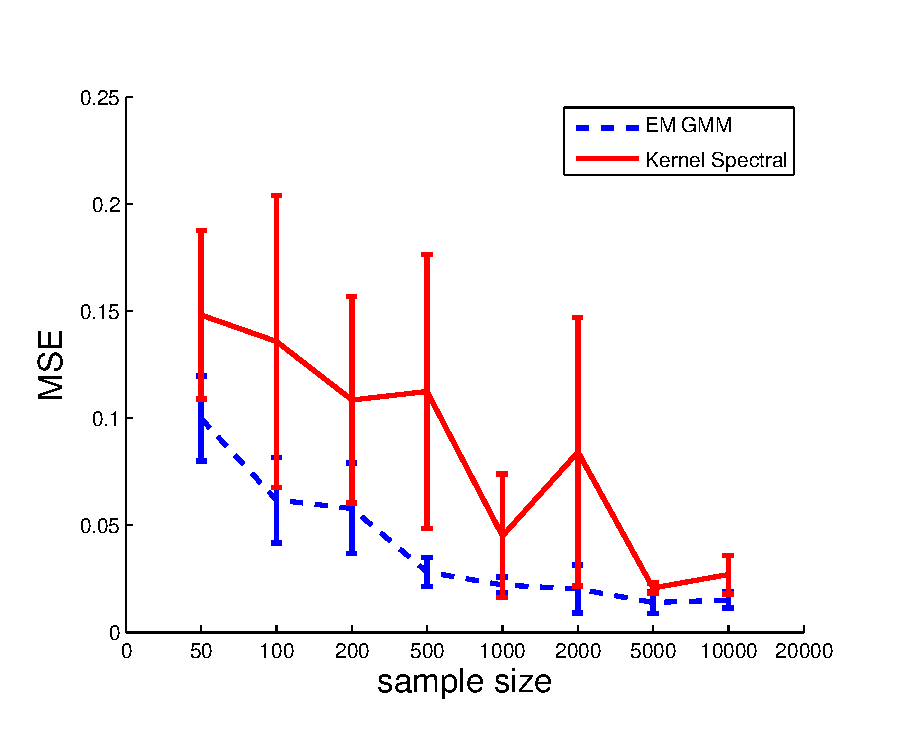
\includegraphics[width=0.32\textwidth]{figure/diff_gauss_k_8_view_3.pdf}
	}
	\subfigure[View 2]{
		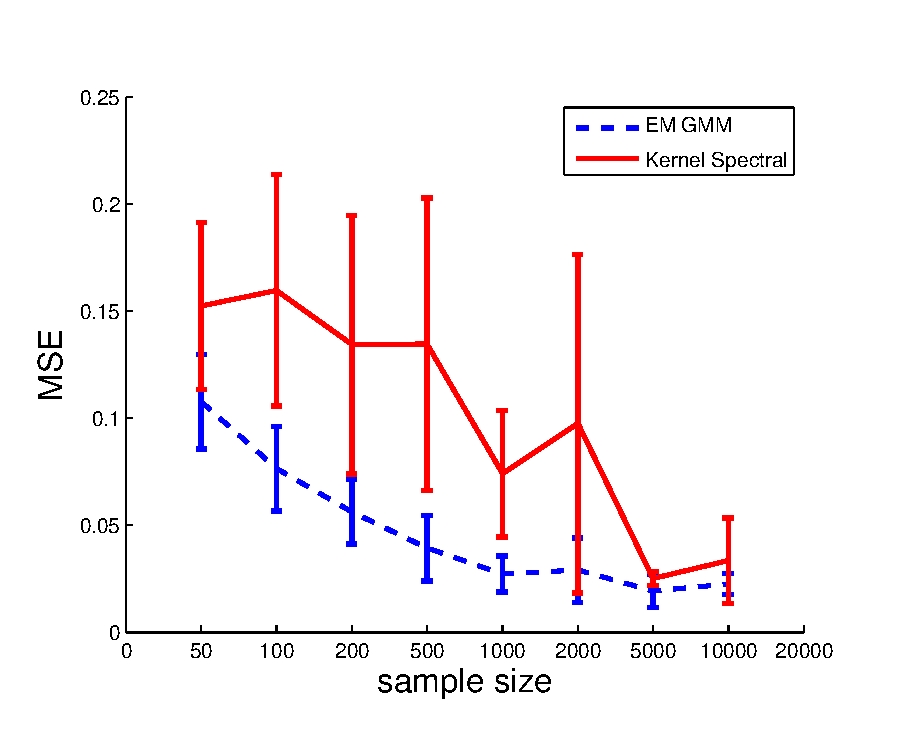
\includegraphics[width=0.32\textwidth]{figure/diff_gauss_k_8_view_2.pdf}
	}
	\subfigure[View 3]{
		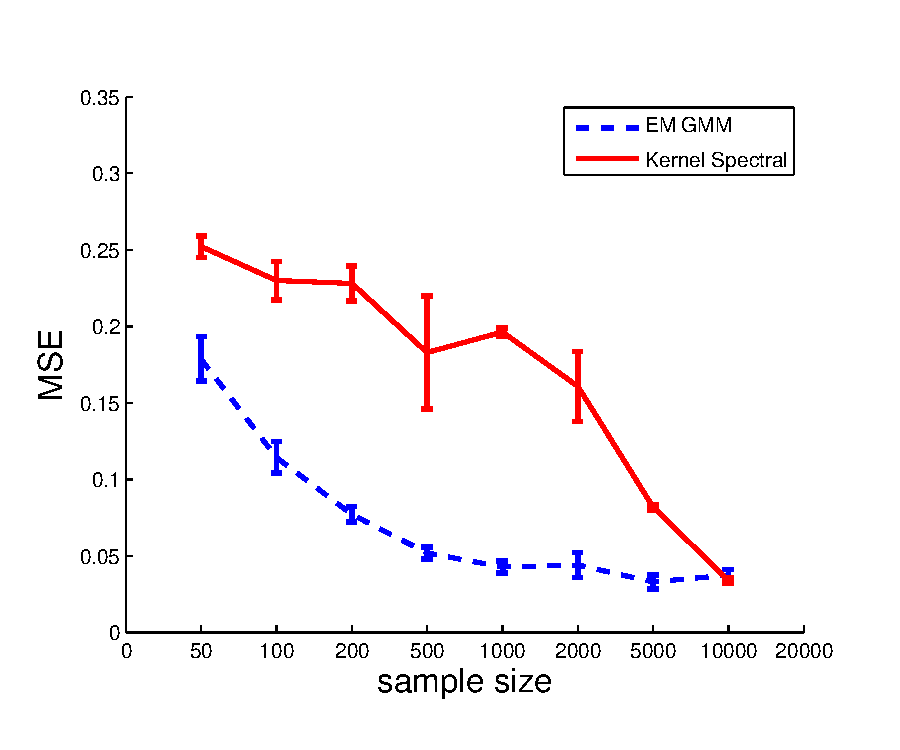
\includegraphics[width=0.32\textwidth]{figure/diff_gauss_k_8_view_1.pdf}
	}
\caption{The empirical results on synthetic dataset with different 8 Gaussian components in eavh view measured by the $l2$-norm between marginal distribution and ground-truth for each view.}
\end{figure}


\begin{figure}
	\subfigure[2 components]{
		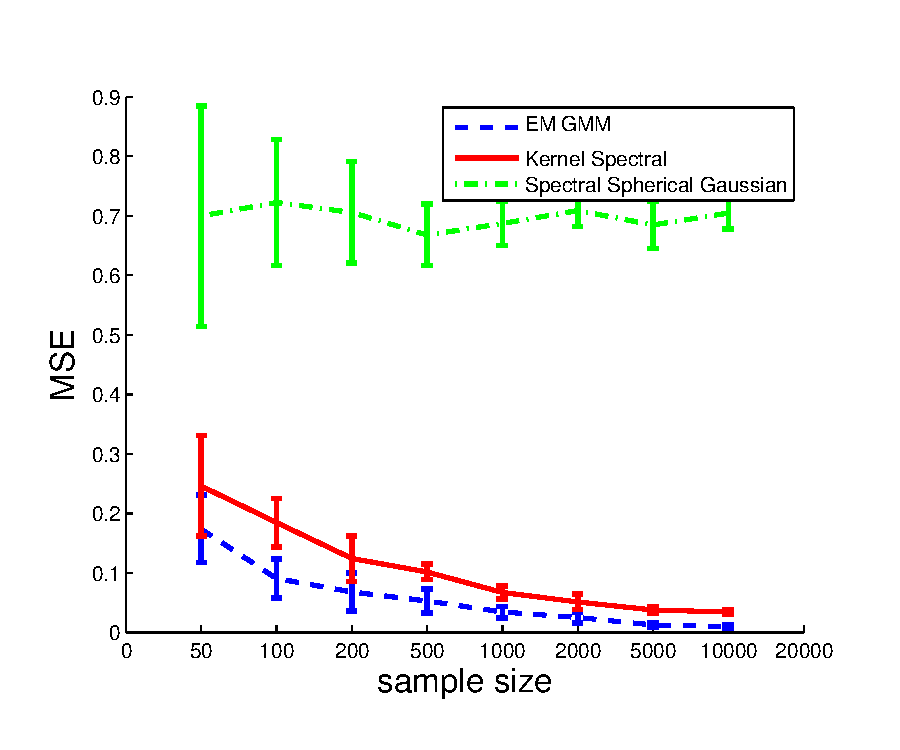
\includegraphics[width=0.23\textwidth]{figure/sym_gauss_k_2.pdf}
	}
	\subfigure[3 components]{
		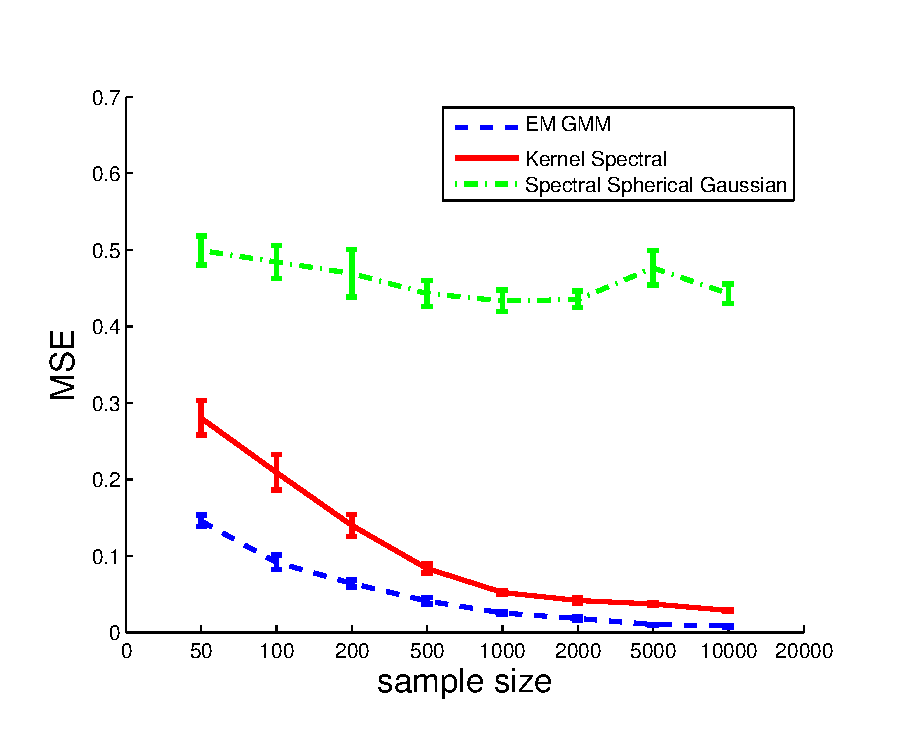
\includegraphics[width=0.23\textwidth]{figure/sym_gauss_k_3.pdf}
	}
	\subfigure[4 components]{
		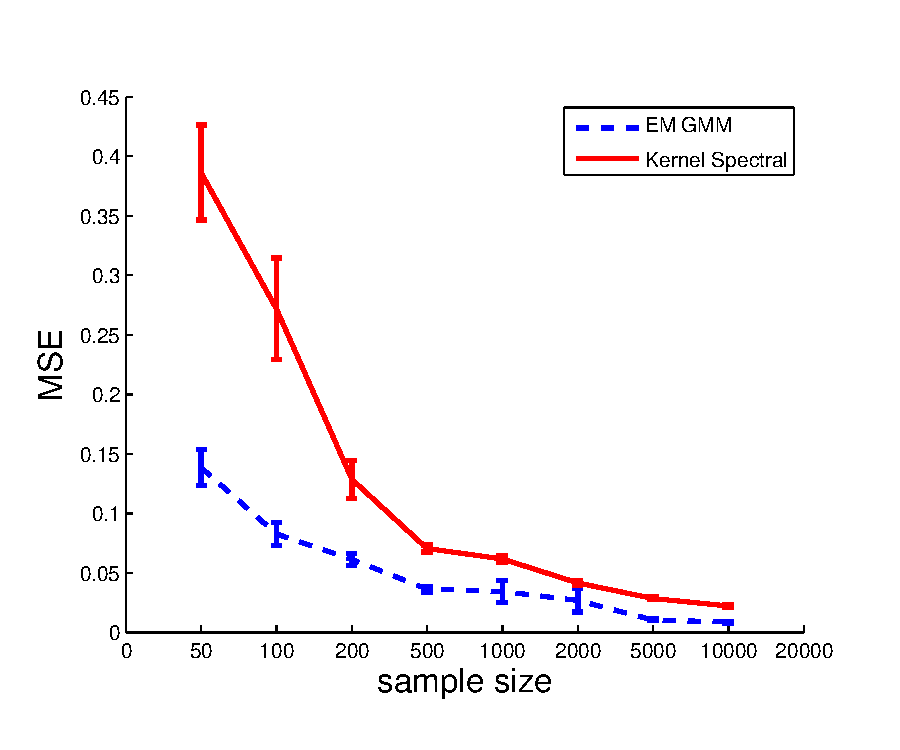
\includegraphics[width=0.23\textwidth]{figure/sym_gauss_k_4.pdf}
	}
	\subfigure[8 components]{
		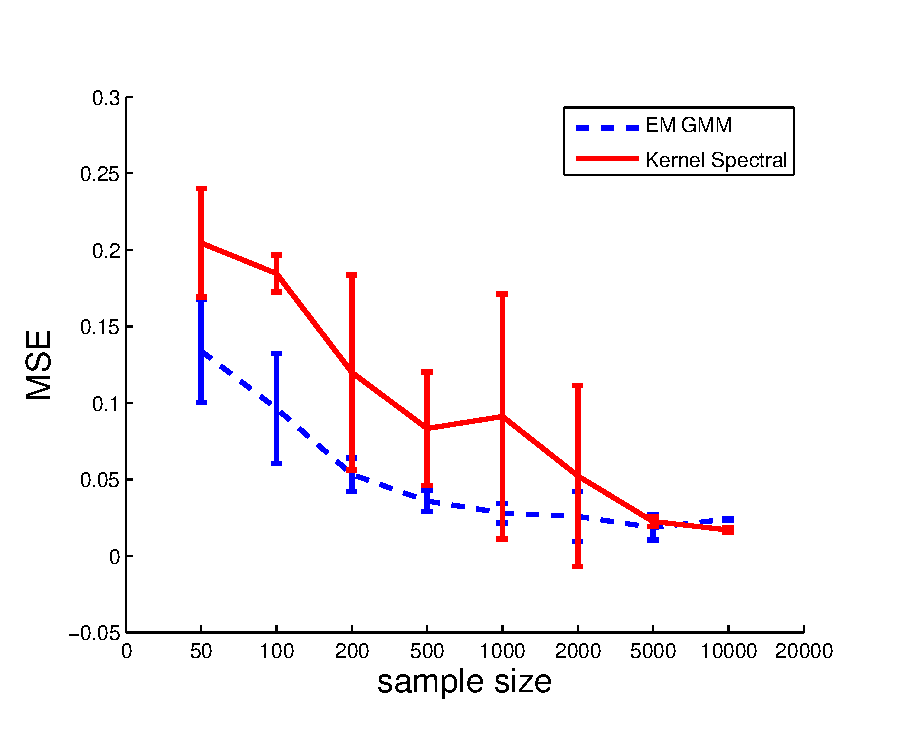
\includegraphics[width=0.23\textwidth]{figure/sym_gauss_k_8.pdf}
	}
\caption{The empirical results on synthetic dataset with same Gaussian components in eavh view measured by the $l2$-norm between marginal distribution and ground-truth.}
\end{figure}


\begin{figure}
	\subfigure[View 1]{
		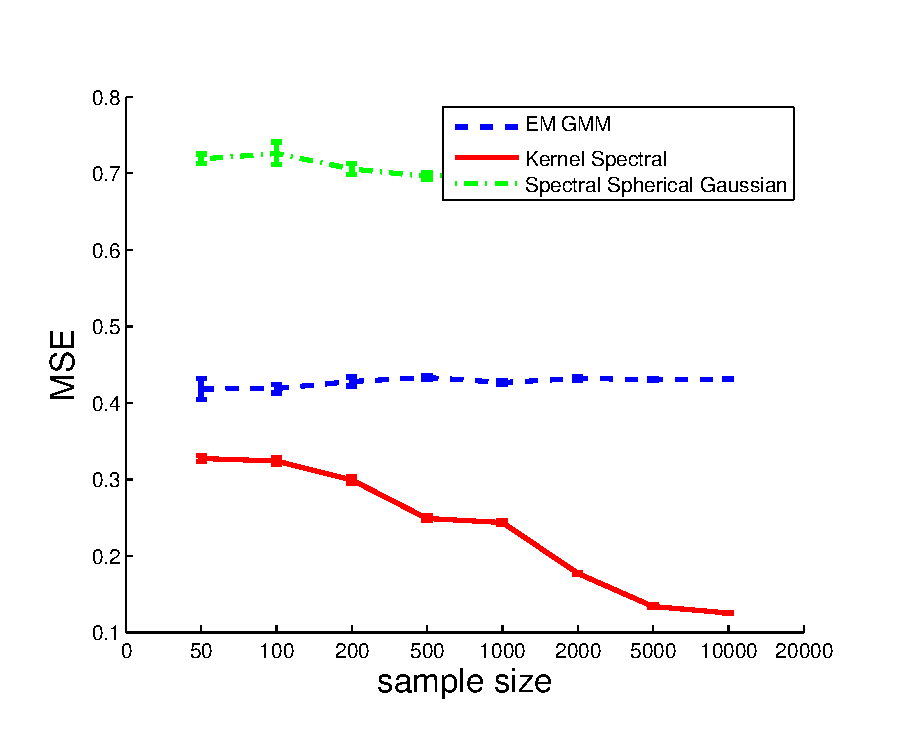
\includegraphics[width=0.32\textwidth]{figure/diff_heter_k_2_view_3.pdf}
	}
	\subfigure[View 2]{
		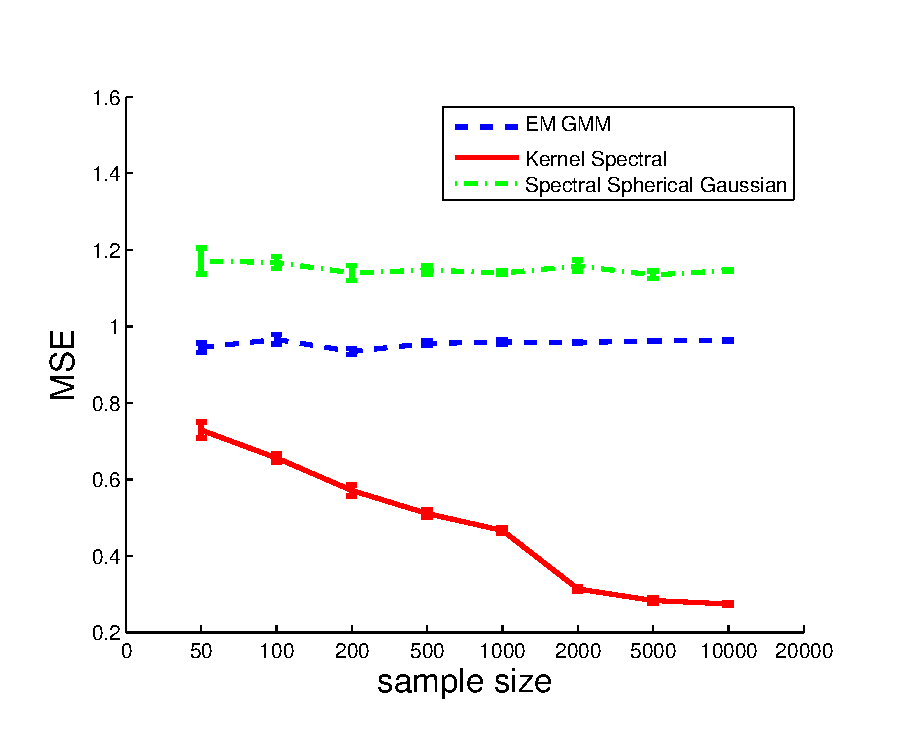
\includegraphics[width=0.32\textwidth]{figure/diff_heter_k_2_view_2.pdf}
	}
	\subfigure[View 3]{
		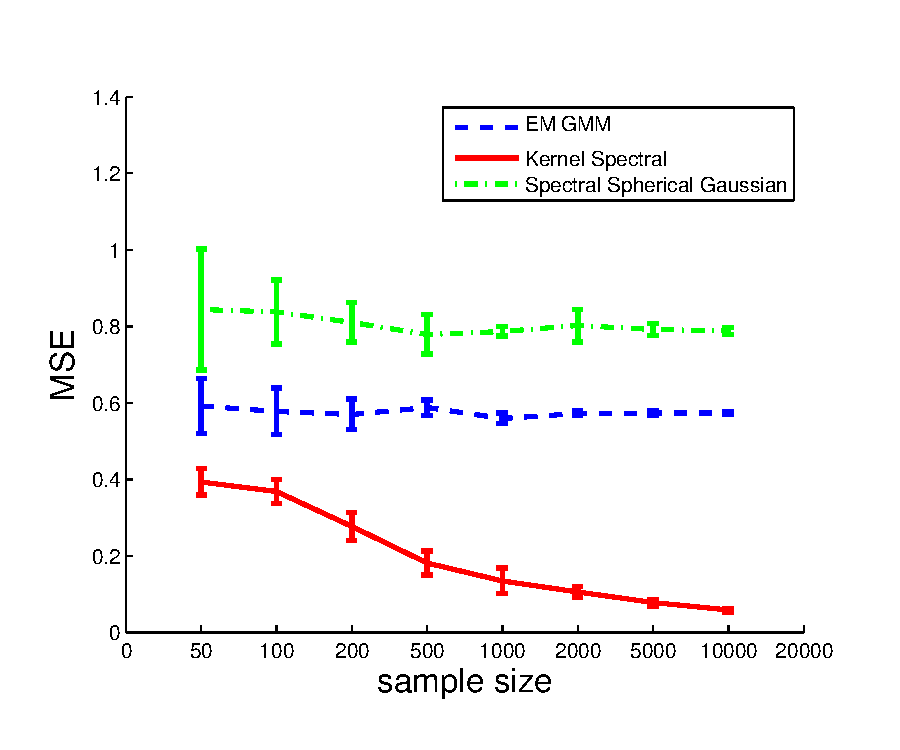
\includegraphics[width=0.32\textwidth]{figure/diff_heter_k_2_view_1.pdf}
	}
\caption{The empirical results on synthetic dataset with different 2 Gaussian/Gamma components in eavh view measured by the $l2$-norm between marginal distribution and ground-truth for each view.}
\end{figure}


\begin{figure}
	\subfigure[View 1]{
		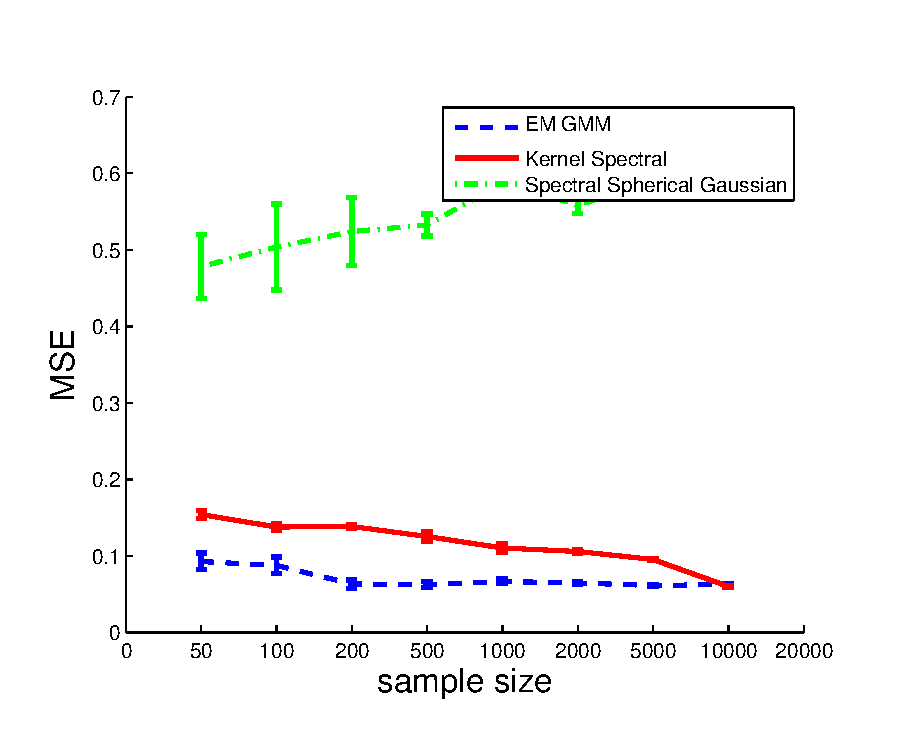
\includegraphics[width=0.32\textwidth]{figure/diff_heter_k_3_view_3.pdf}
	}
	\subfigure[View 2]{
		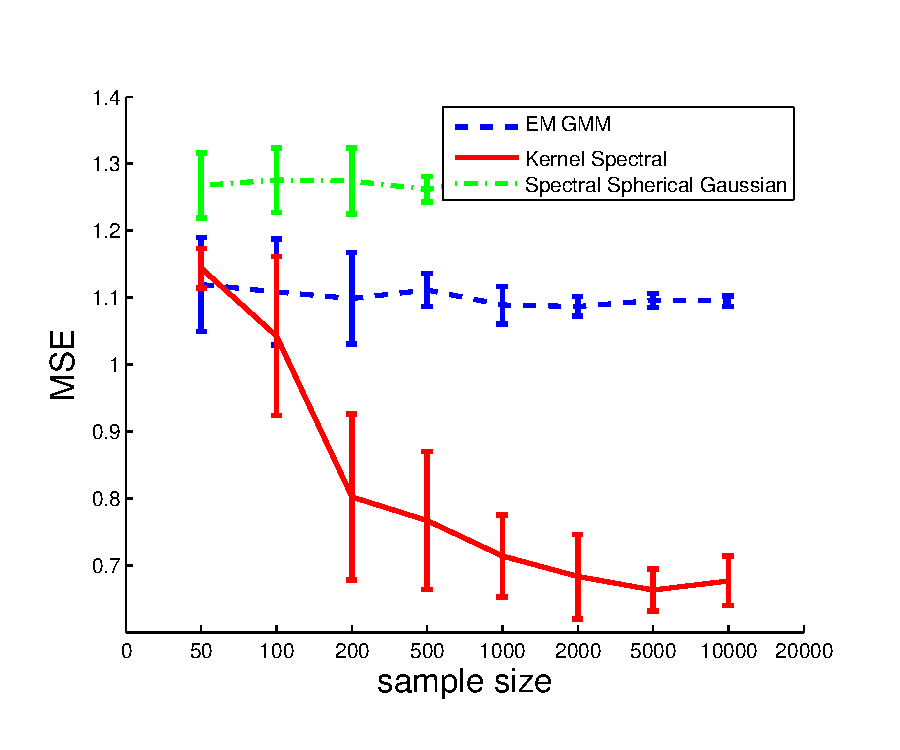
\includegraphics[width=0.32\textwidth]{figure/diff_heter_k_3_view_2.pdf}
	}
	\subfigure[View 3]{
		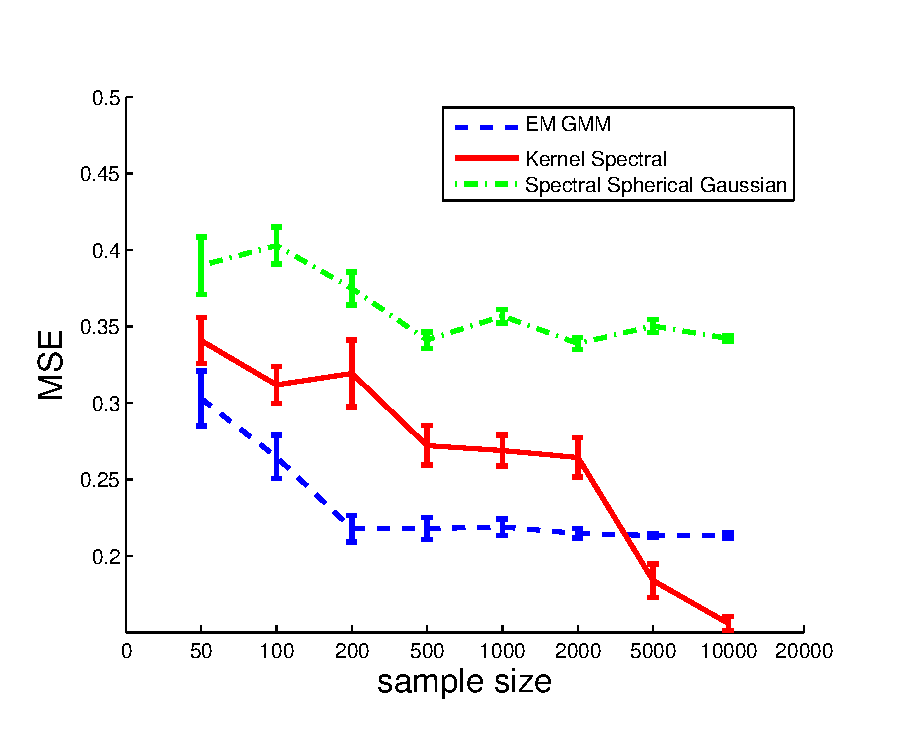
\includegraphics[width=0.32\textwidth]{figure/diff_heter_k_3_view_1.pdf}
	}
\caption{The empirical results on synthetic dataset with different 3 Gaussian/Gamma components in eavh view measured by the $l2$-norm between marginal distribution and ground-truth for each view.}
\end{figure}

\begin{figure}
	\subfigure[View 1]{
		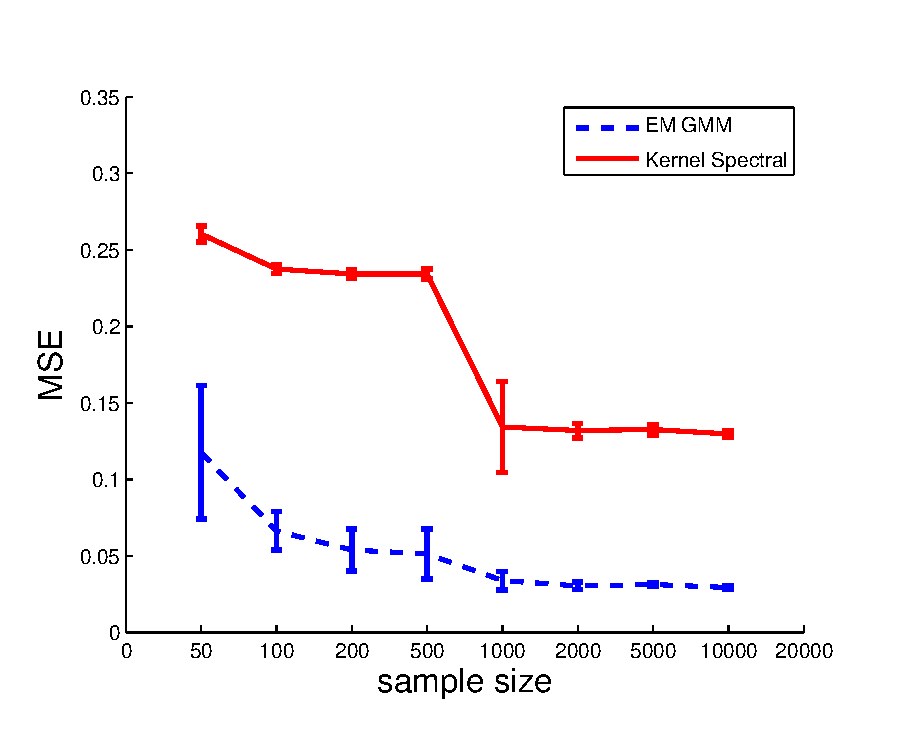
\includegraphics[width=0.32\textwidth]{figure/diff_heter_k_4_view_3.pdf}
	}
	\subfigure[View 2]{
		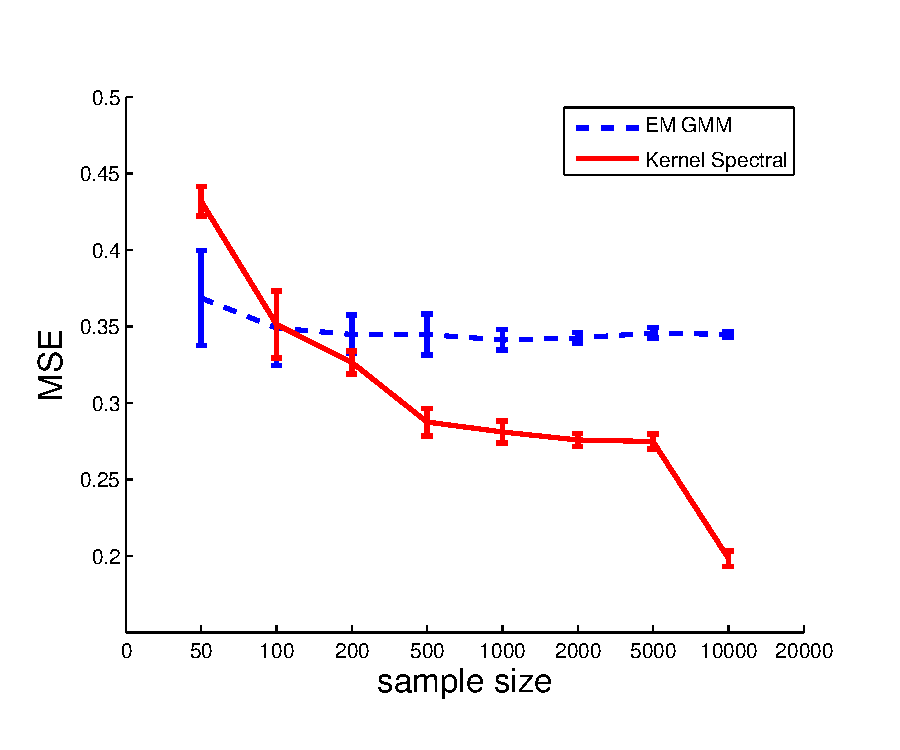
\includegraphics[width=0.32\textwidth]{figure/diff_heter_k_4_view_2.pdf}
	}
	\subfigure[View 3]{
		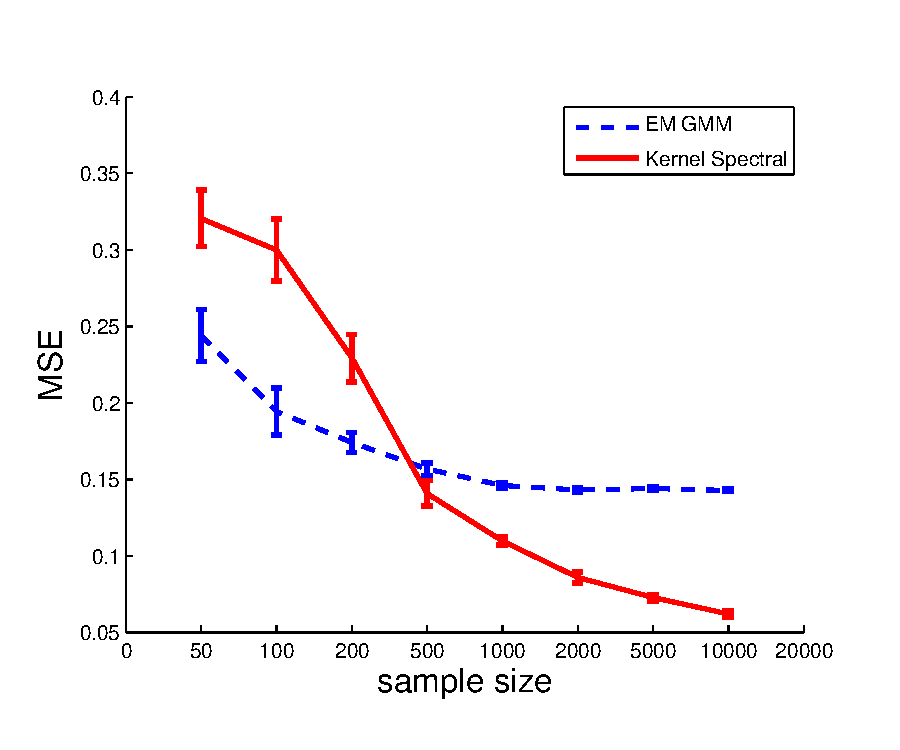
\includegraphics[width=0.32\textwidth]{figure/diff_heter_k_4_view_1.pdf}
	}
\caption{The empirical results on synthetic dataset with different 4 Gaussian/Gamma components in eavh view measured by the $l2$-norm between marginal distribution and ground-truth for each view.}
\end{figure}

\begin{figure}
	\subfigure[View 1]{
		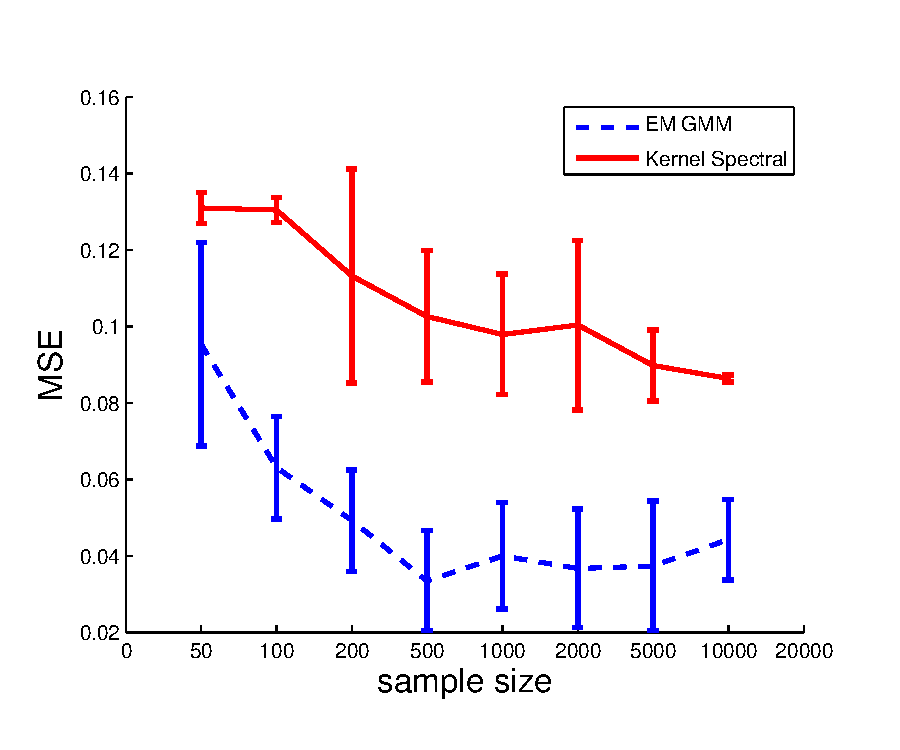
\includegraphics[width=0.32\textwidth]{figure/diff_heter_k_8_view_3.pdf}
	}
	\subfigure[View 2]{
		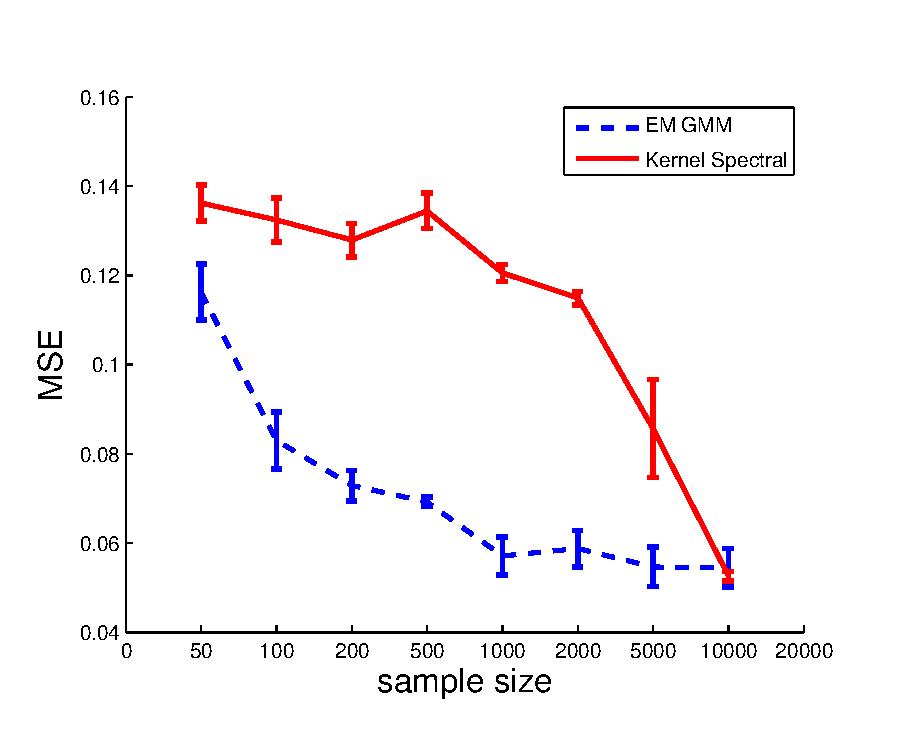
\includegraphics[width=0.32\textwidth]{figure/diff_heter_k_8_view_2.pdf}
	}
	\subfigure[View 3]{
		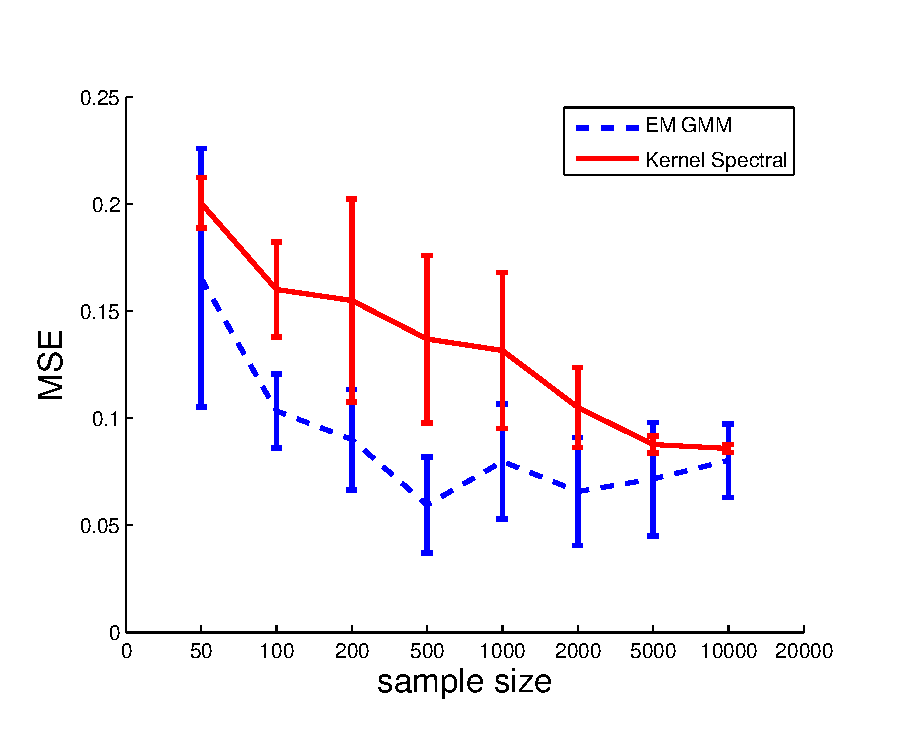
\includegraphics[width=0.32\textwidth]{figure/diff_heter_k_8_view_1.pdf}
	}
\caption{The empirical results on synthetic dataset with different 8 Gaussian/Gamma components in eavh view measured by the $l2$-norm between marginal distribution and ground-truth for each view.}
\end{figure}


\begin{figure}
	\subfigure[2 components]{
		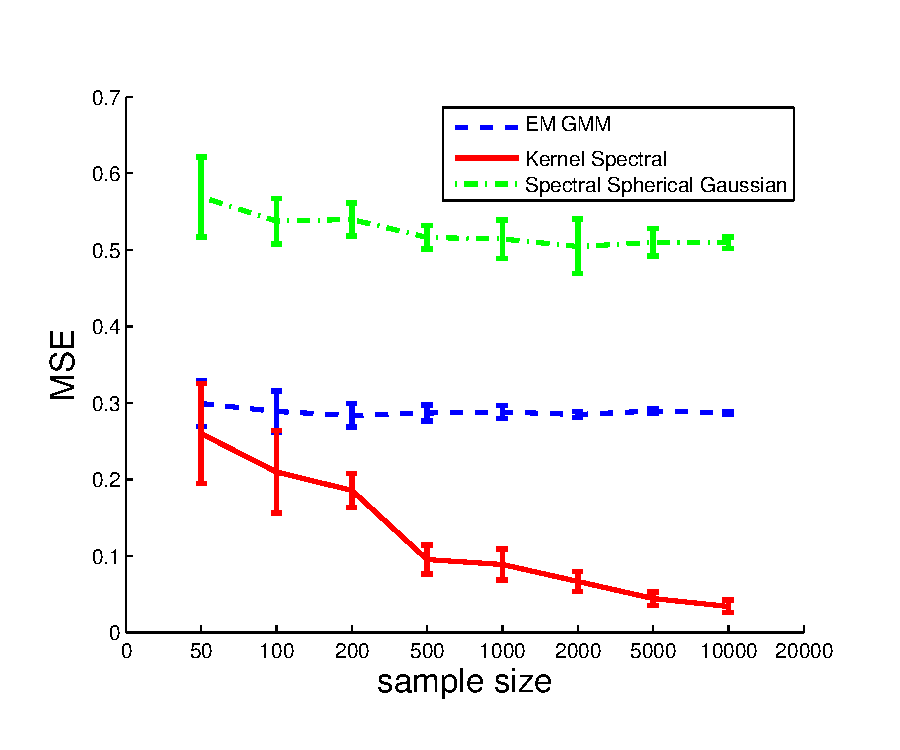
\includegraphics[width=0.23\textwidth]{figure/sym_heter_k_2.pdf}
	}
	\subfigure[3 components]{
		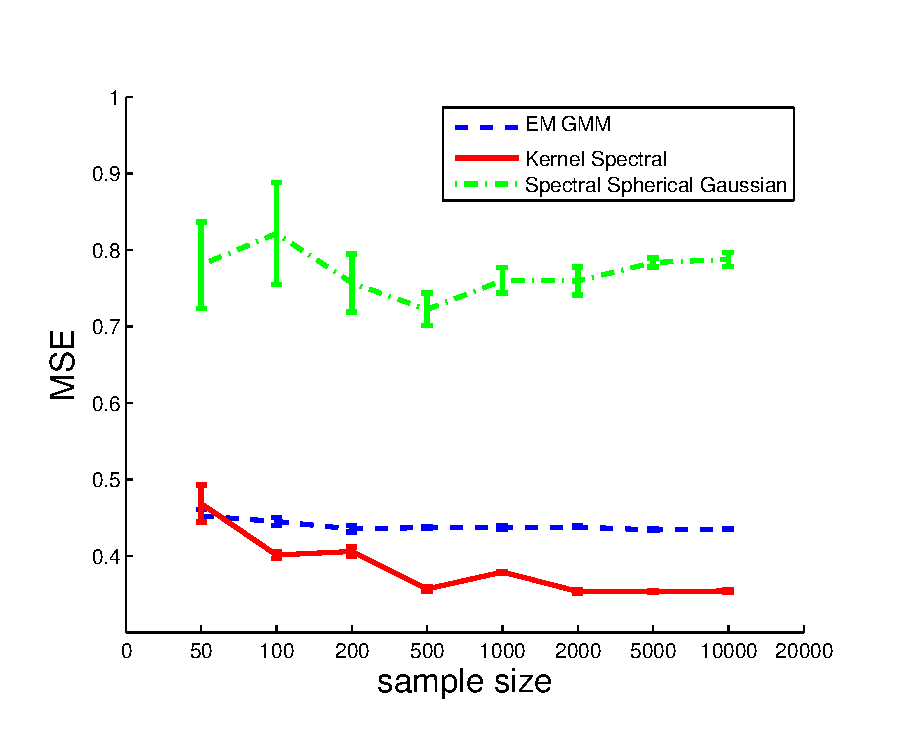
\includegraphics[width=0.23\textwidth]{figure/sym_heter_k_3.pdf}
	}
	\subfigure[4 components]{
		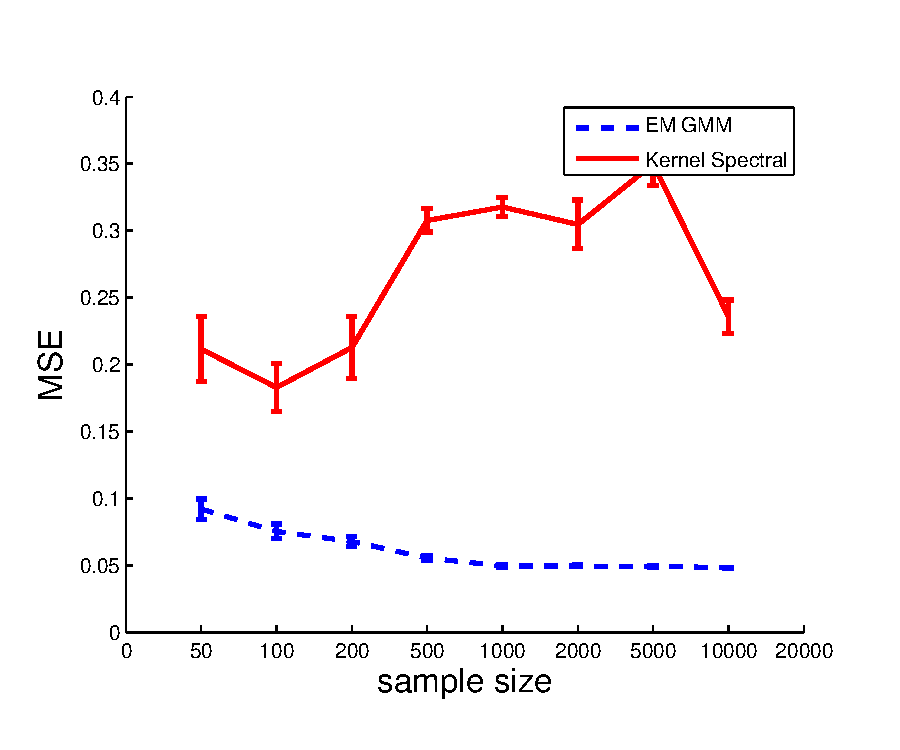
\includegraphics[width=0.23\textwidth]{figure/sym_heter_k_4.pdf}
	}
	\subfigure[8 components]{
		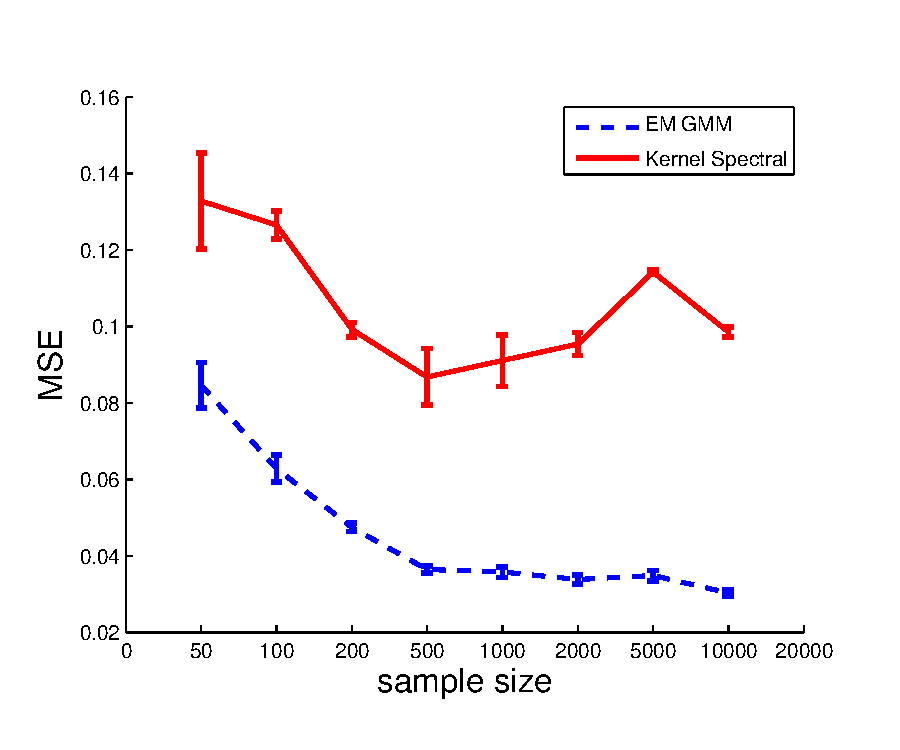
\includegraphics[width=0.23\textwidth]{figure/sym_heter_k_8.pdf}
	}
\caption{The empirical results on synthetic dataset with same Gaussian/Gamma components in eavh view measured by the $l2$-norm between marginal distribution and ground-truth.}
\end{figure}





\begin{figure}
	\subfigure[View 1]{
		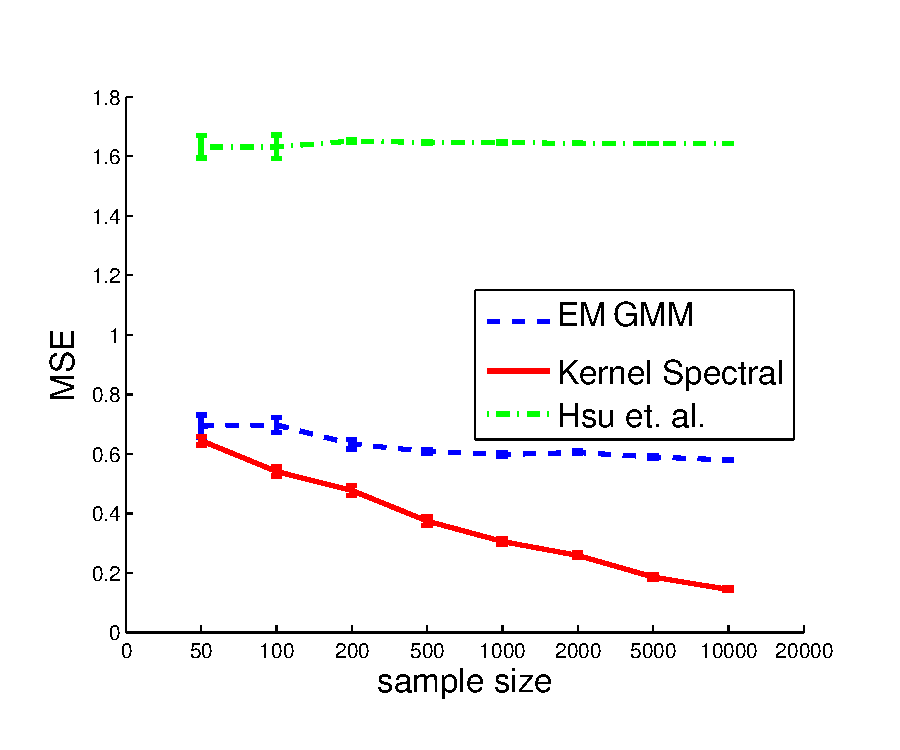
\includegraphics[width=0.32\textwidth]{figure/sp_diff_heter_k_2_view_3.pdf}
	}
	\subfigure[View 2]{
		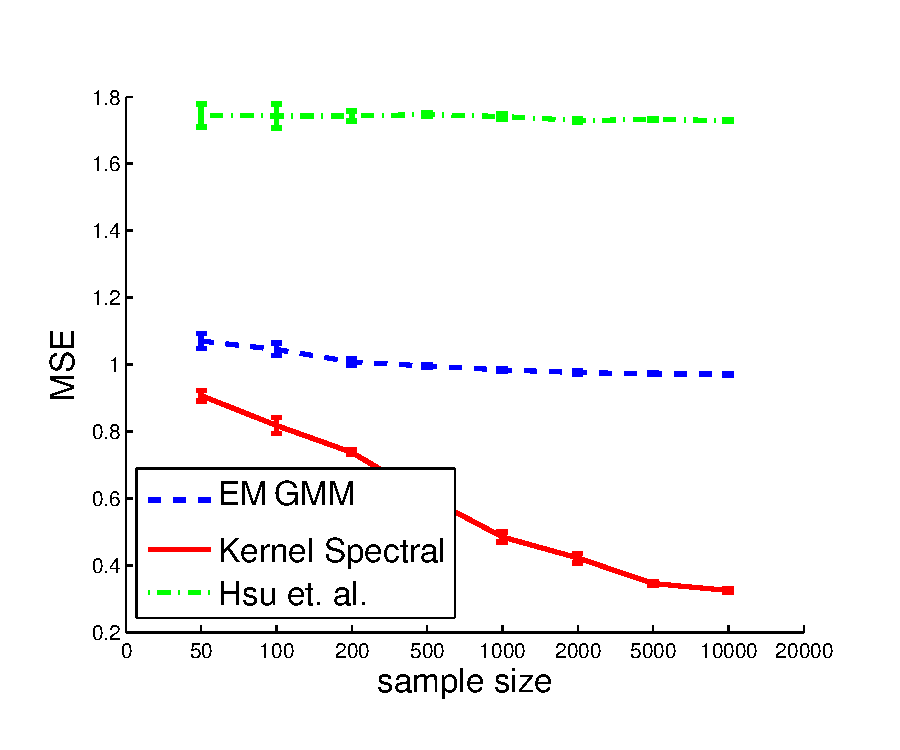
\includegraphics[width=0.32\textwidth]{figure/sp_diff_heter_k_2_view_2.pdf}
	}
	\subfigure[View 3]{
		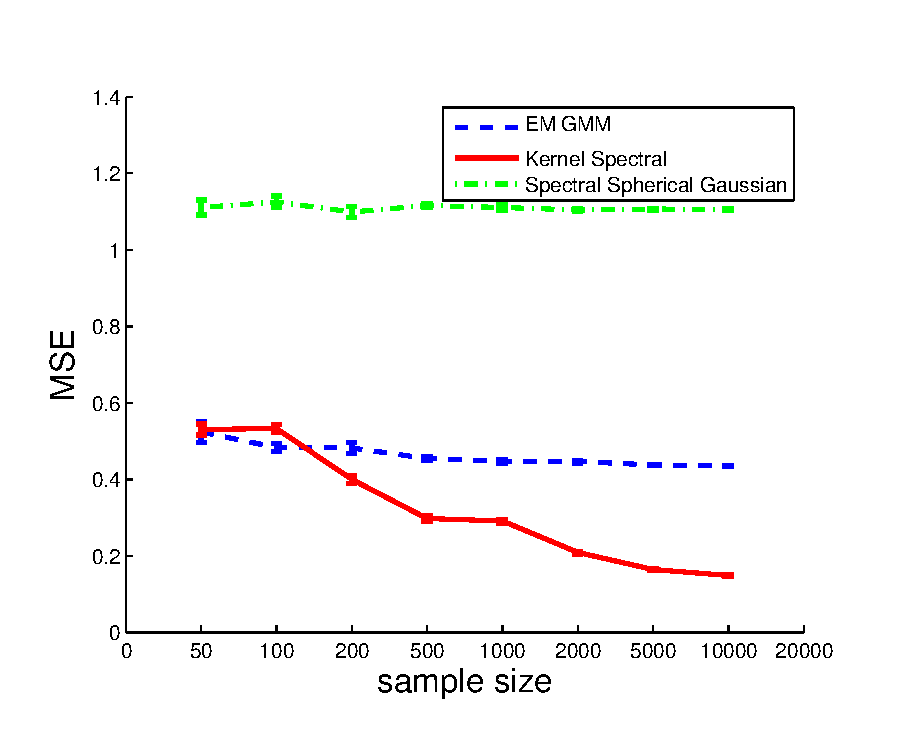
\includegraphics[width=0.32\textwidth]{figure/sp_diff_heter_k_2_view_1.pdf}
	}
\caption{The empirical results on synthetic dataset with different 2 Gaussian/Gamma components in eavh view measured by the weighted sum of $l2$-norm between the component distribution and ground-truth for each view.}
\end{figure}


\begin{figure}
	\subfigure[View 1]{
		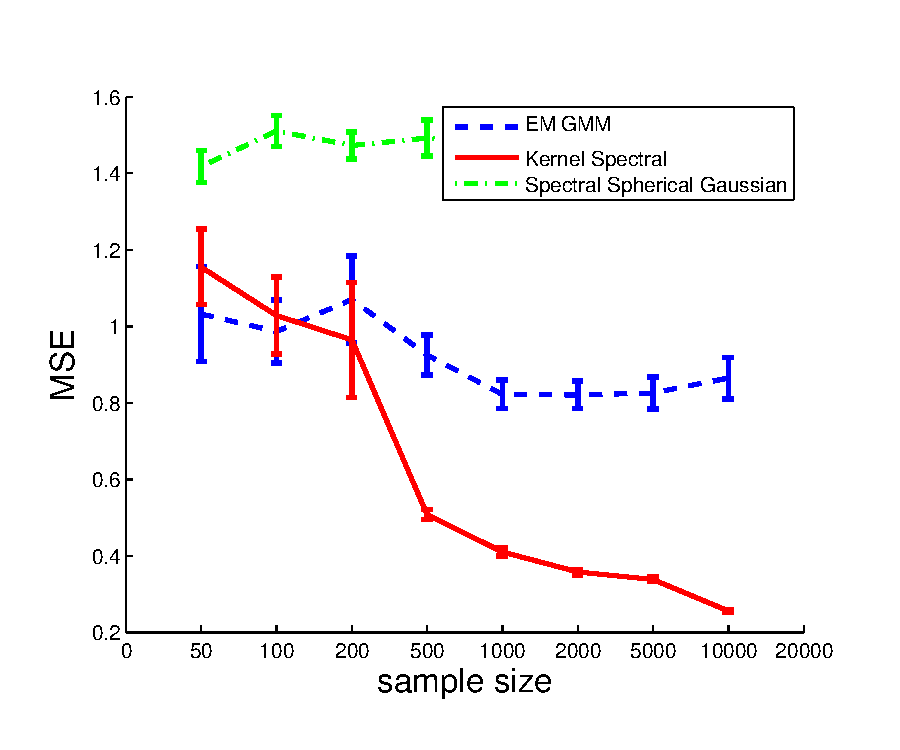
\includegraphics[width=0.32\textwidth]{figure/sp_diff_heter_k_3_view_3.pdf}
	}
	\subfigure[View 2]{
		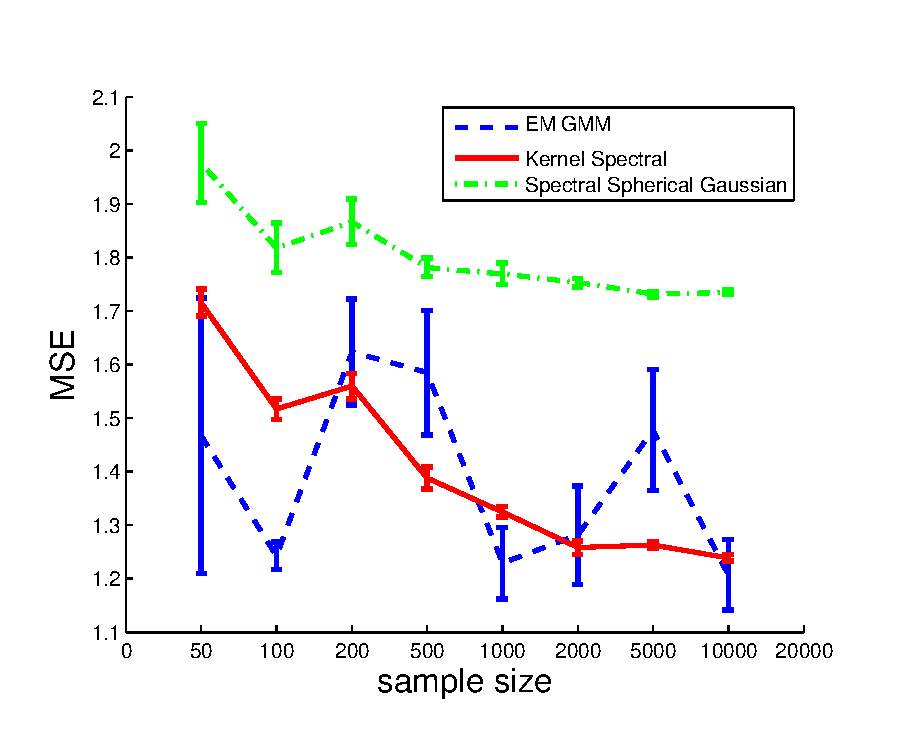
\includegraphics[width=0.32\textwidth]{figure/sp_diff_heter_k_3_view_2.pdf}
	}
	\subfigure[View 3]{
		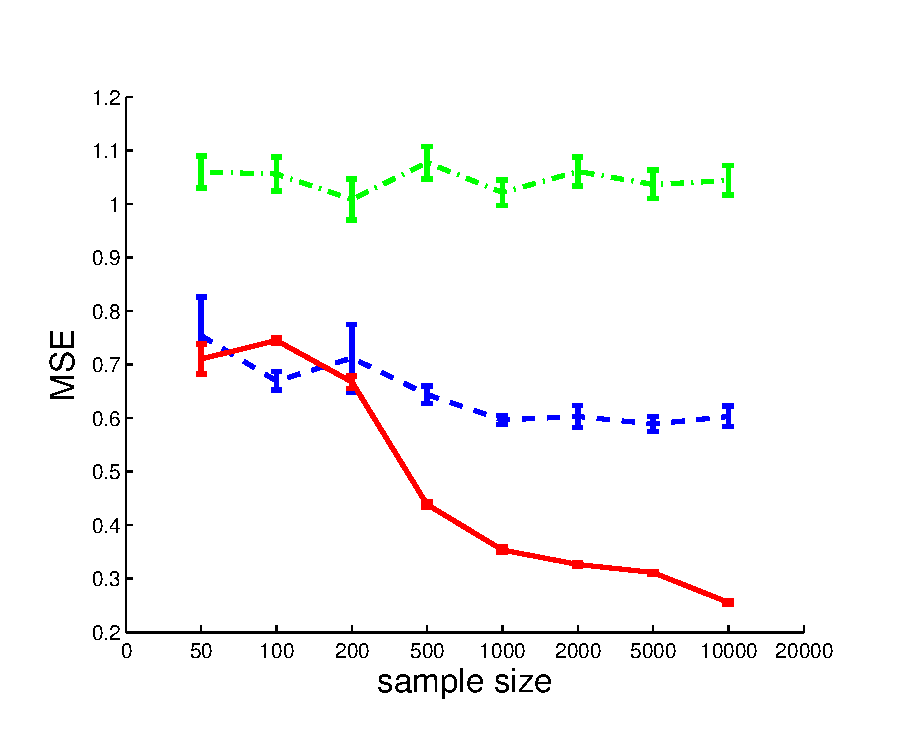
\includegraphics[width=0.32\textwidth]{figure/sp_diff_heter_k_3_view_1.pdf}
	}
\caption{The empirical results on synthetic dataset with different 3 Gaussian/Gamma components in eavh view measured by the $l2$-norm between marginal distribution and ground-truth for each view.}
\end{figure}

\begin{figure}
	\subfigure[View 1]{
		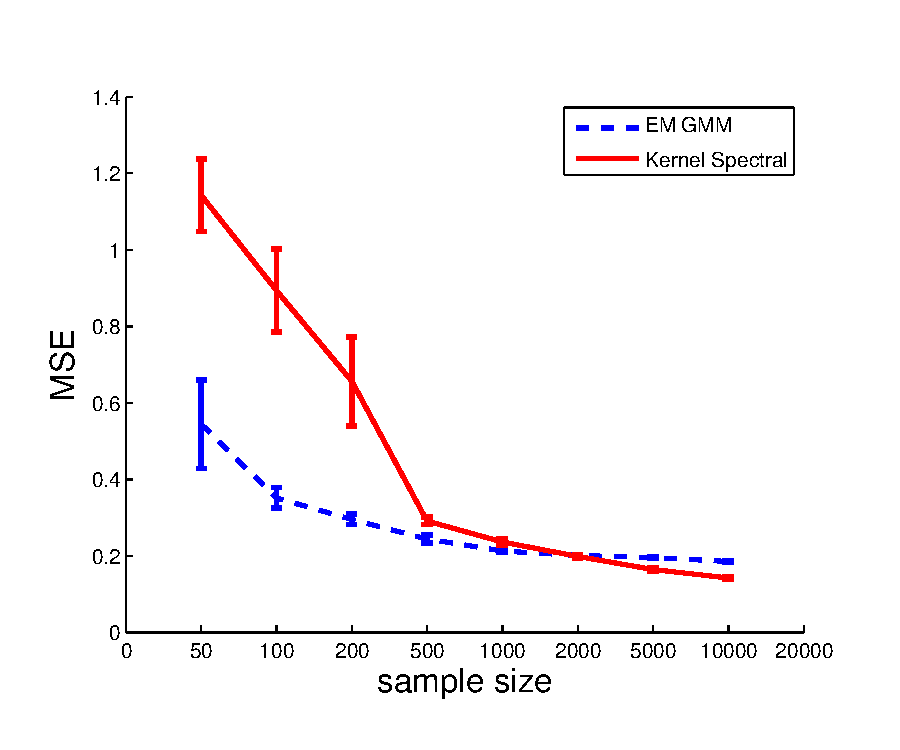
\includegraphics[width=0.32\textwidth]{figure/sp_diff_heter_k_4_view_3.pdf}
	}
	\subfigure[View 2]{
		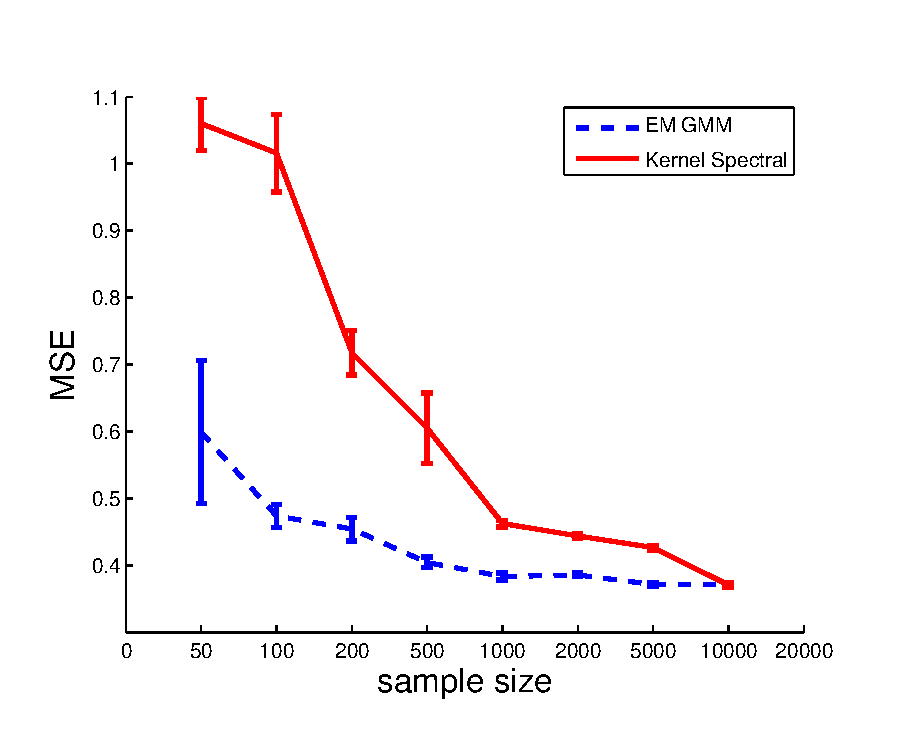
\includegraphics[width=0.32\textwidth]{figure/sp_diff_heter_k_4_view_2.pdf}
	}
	\subfigure[View 3]{
		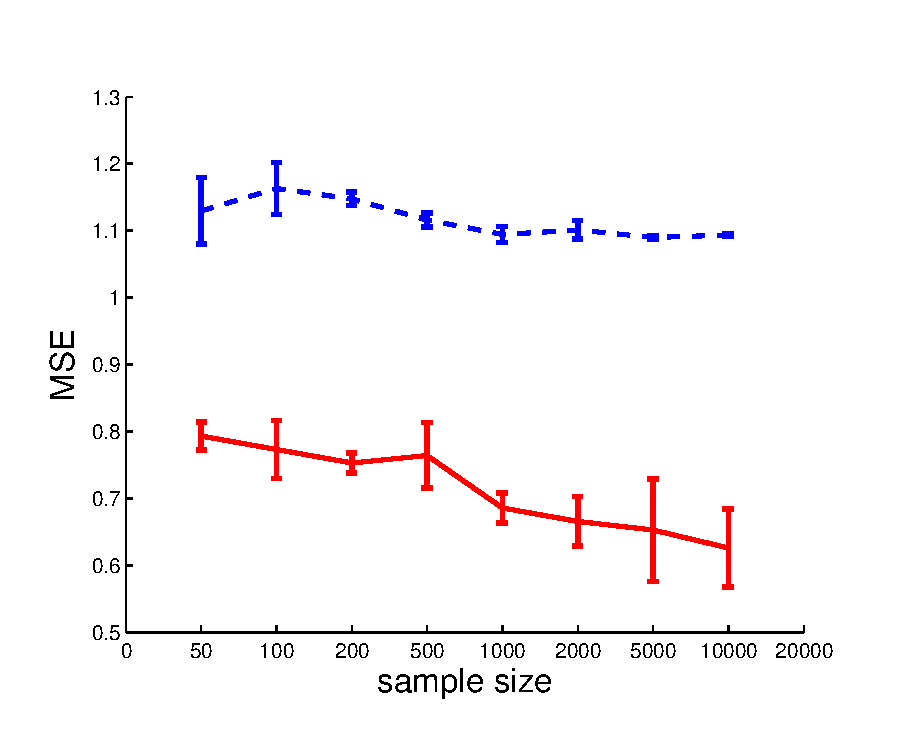
\includegraphics[width=0.32\textwidth]{figure/sp_diff_heter_k_4_view_1.pdf}
	}
\caption{The empirical results on synthetic dataset with different 4 Gaussian/Gamma components in eavh view measured by the weighted sum of $l2$-norm between the component distribution and ground-truth for each view.}
\end{figure}

\begin{figure}
	\subfigure[View 1]{
		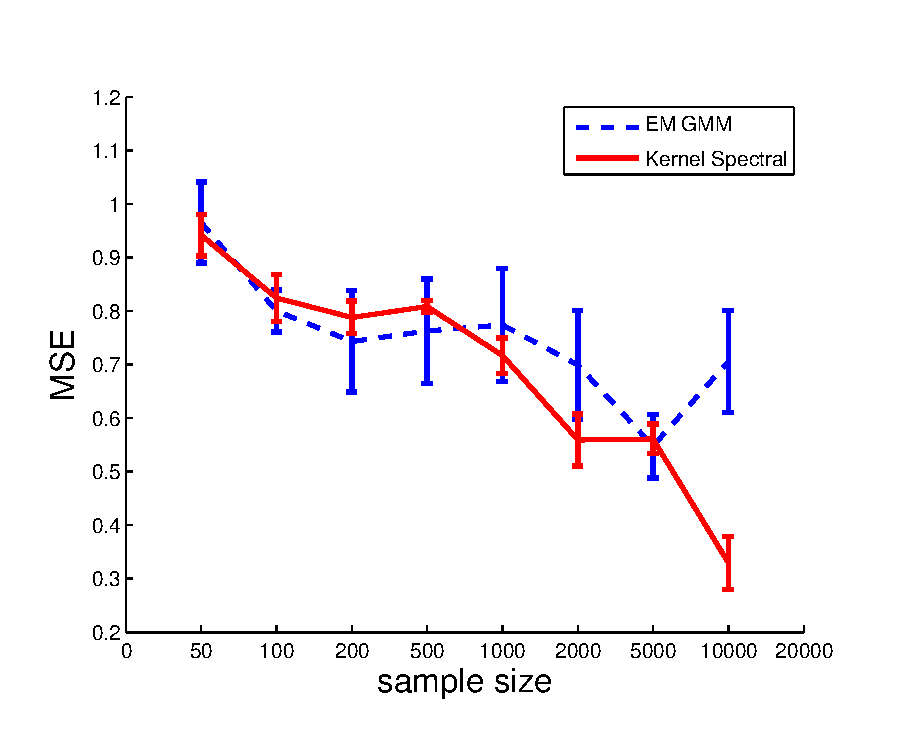
\includegraphics[width=0.32\textwidth]{figure/sp_diff_heter_k_8_view_3.pdf}
	}
	\subfigure[View 2]{
		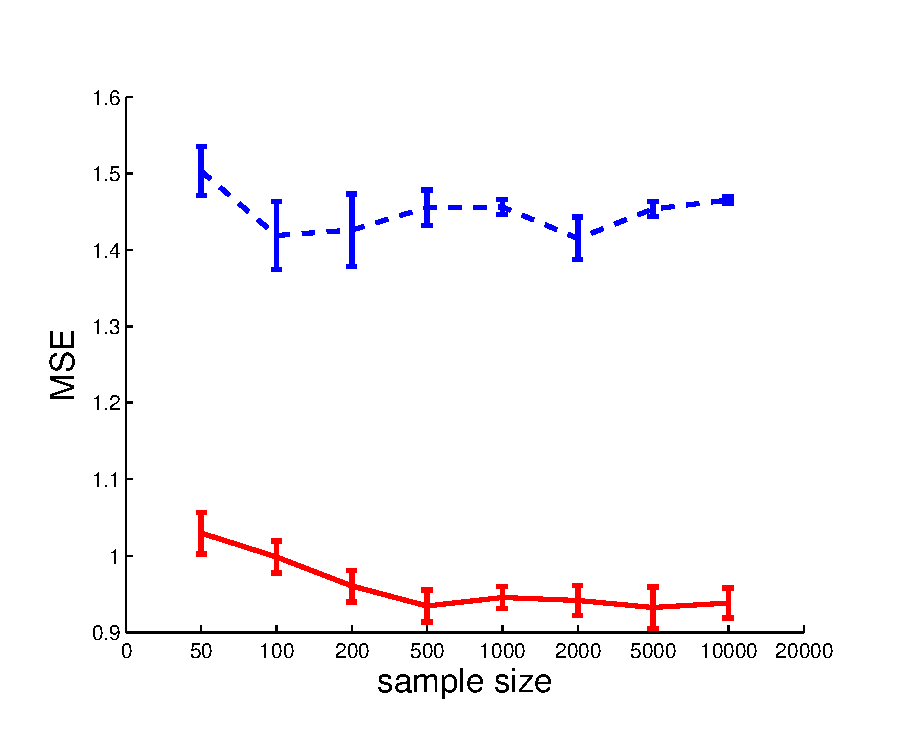
\includegraphics[width=0.32\textwidth]{figure/sp_diff_heter_k_8_view_2.pdf}
	}
	\subfigure[View 3]{
		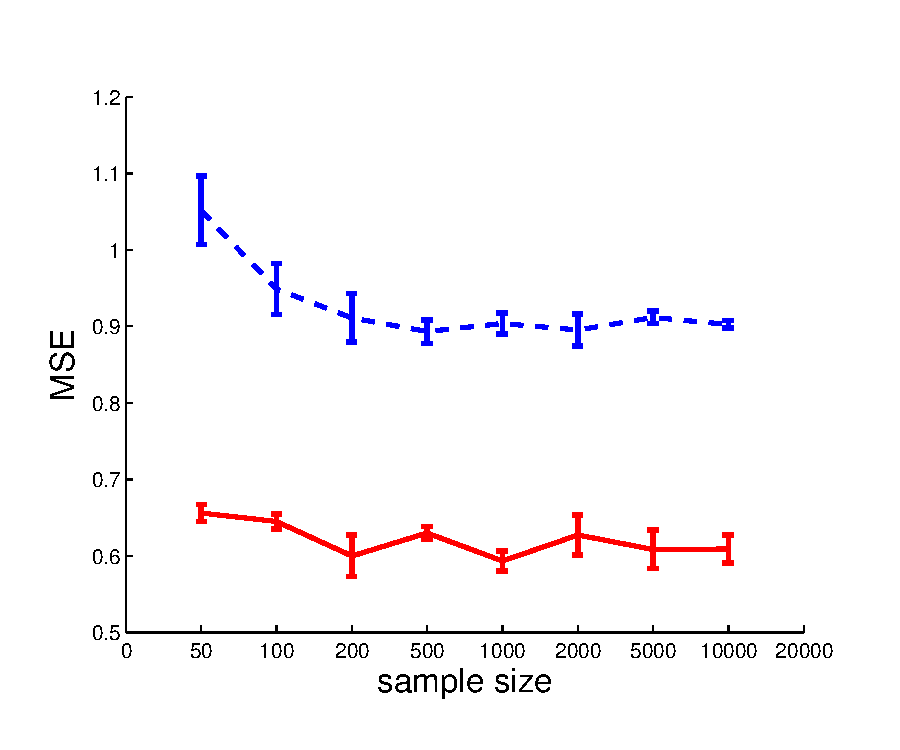
\includegraphics[width=0.32\textwidth]{figure/sp_diff_heter_k_8_view_1.pdf}
	}
\caption{The empirical results on synthetic dataset with different 8 Gaussian/Gamma components in eavh view measured by the weighted sum of $l2$-norm between the component distribution and ground-truth for each view.}
\end{figure}


\bibliography{mlv_kernel}
\bibliographystyle{icml2013}

\end{document}
